\documentclass[conference]{IEEEtran}
\IEEEoverridecommandlockouts

\usepackage{amsmath,amssymb,amsfonts}
\usepackage{booktabs}
\usepackage{array}
\usepackage{multirow}
\usepackage{graphicx}
\graphicspath{{figures/imported/}{manuscript/figures/imported/}}
\usepackage{cite}
\usepackage{url}

\newcommand{\BSC}{\ensuremath{\mathrm{BSC}_{6}}}
\newcommand{\R}{\mathbb{R}}
\newcommand{\Ind}{\mathbf{1}}

\title{On the Edge of Stability: Spiking Reservoir State-Space Encoding of Affective EEG}

\author{
\IEEEauthorblockN{Andrew A. Lane\IEEEauthorrefmark{1}, Wendy Tang\IEEEauthorrefmark{1}, and Brady D. Nelson\IEEEauthorrefmark{2}}
\IEEEauthorblockA{\IEEEauthorrefmark{1}Department of Electrical and Computer Engineering, Stony Brook University, Stony Brook, NY, USA}
\IEEEauthorblockA{\IEEEauthorrefmark{2}Department of Psychology, Stony Brook University, Stony Brook, NY, USA}
}

\begin{document}
\maketitle

\begin{abstract}
How a representation of affective event-related potentials (ERPs) degrades under perturbation can depend on the evaluation protocol as much as on the representation. We encode affective ERPs with a fixed leaky integrate-and-fire spiking reservoir operated near its measured edge of stability ($\rho^\ast\approx0.82$, below the echo-state heuristic $\rho=1$; removing the recurrence costs $0.049$ balanced accuracy, BA, $95\%$ CI $[-0.098,-0.002]$) and compare it with band-power, ERP-window, and trained EEGNet representations under subject-grouped validation with subject-level uncertainty. Two scoring effects distort channel-dropout comparisons: raw retention rewards encoders near the chance floor, and zero-filling a dropped channel before standardization is not invariant to re-centering the features, so at $30\%$ dropout it halves the measured lead of ERP-window features over the near-centered reservoir ($+0.05$ versus $+0.09$ to $+0.11$ BA), and on DEAP the fill rule moves band-power BA by up to $0.11$. When the raw signal itself is corrupted, identically for every encoder, ERP-window features stay ahead of the reservoir, whose fill invariance does not survive removal of half the electrodes, and channel-dropout augmentation more than halves EEGNet's loss to electrode removal. We recommend reporting absolute accuracy with subject-level uncertainty, stating and varying the fill rule, and reporting trained models with and without augmentation.
\end{abstract}


\begin{IEEEkeywords}
EEG, event-related potentials, spiking neural networks, reservoir computing, affective computing, neuromorphic computing, ARSPI-Net.
\end{IEEEkeywords}

\section{Introduction}
Electroencephalographic event-related potentials (ERPs) provide millisecond-scale measurements of evoked neural dynamics, but the recorded waveform is a noisy, low-dimensional, and subject-dependent projection of an unobserved neural process \cite{makeig2002dynamic,blankertz2011singletrial}. A representation may separate affective conditions under one protocol while preserving little usable structure after amplitude noise, temporal misalignment, or channel loss.

Endpoint accuracy alone also says little about what a representation preserves, which matters for spiking encodings. Fixed recurrent reservoirs and spiking networks provide nonlinear temporal expansions \cite{maass2002real,lukosevicius2009reservoir}, but EEG/ERP studies often treat them primarily as classifiers \cite{gong2023sglnet,craik2019deep}, and their spike-count features are rarely examined as perturbation-sensitive temporal measurements. How such encodings change under perturbation has received little attention, even though preprocessing, acquisition, and electrode-loss choices can materially change EEG representation performance \cite{delpup2025preprocessing,chiang2023depression,guo2025mma}. Channel-dropout comparisons that zero-fill a dropped channel also do not account for the coordinate origin of the features, which, as we show, can change the measured result.

This paper evaluates whether channel-dropout robustness rankings for affective-ERP representations are stable under reasonable changes to the scoring protocol. We compare spectral band-power, ERP-window amplitudes, a fixed leaky integrate-and-fire (LIF) reservoir operated near the edge of its ordered regime and summarized by six spike-count bins (\BSC{}), and a trained EEGNet. The reservoir is not treated as a proposed winner; it is used as a fixed reference whose embedding is nearly zero-centered and whose dynamics are not retrained under perturbation. The contributions are:
\begin{enumerate}
    \item A subject-grouped comparison of affective-ERP representations under electrode removal, amplitude noise, and temporal jitter applied identically to every encoder's input, with uncertainty and encoder contrasts from a subject-level bootstrap rather than from folds treated as independent (Secs.~\ref{sec:clean}, \ref{sec:rawsignal}; Tables~\ref{tab:clean}, \ref{tab:rawsignal}).
    \item Quantification of two protocol artifacts in channel-dropout evaluation: raw-retention inflation near the chance floor, and zero-imputation bias for non-centered features, which is not invariant to re-centering (Proposition~1) and is also tested on DEAP (Secs.~\ref{sec:confound}, \ref{sec:perturb}, \ref{sec:deap}).
    \item Paired subject-level evidence that zero-fill halves the measured lead of ERP-window features over the near-centered reservoir, and that channel-dropout augmentation, a training choice, more than halves the trained EEGNet's loss under electrode removal (Table~\ref{tab:dropconf}, Fig.~\ref{fig:impute}, Sec.~\ref{sec:rawsignal}).
    \item A test of the reservoir's operating point: a spectral-radius sweep with a no-recurrence ablation and a measured order parameter places the transition at $\rho^\ast\approx0.82$, below the echo-state heuristic $\rho=1$ and next to the pre-specified $\rho=0.9$, inside a broad accuracy optimum (Fig.~\ref{fig:resdyn}).
\end{enumerate}
Affective categories define the task; the representations and their invariances under perturbation are the object of study.

\section{Related Work}
\label{sec:related}
ERP/EEG analysis commonly uses window amplitudes, Hjorth \cite{hjorth1970eeg} and wavelet/spectral descriptors \cite{subasi2007eeg}, and linear models \cite{blankertz2011singletrial}, which are interpretable through known components such as the P300 and late positive potential \cite{makeig2002dynamic} but can miss nonlinear temporal structure. Reservoir computing offers a complementary view: a fixed high-dimensional recurrent system maps the input to a state trajectory read out by a simple classifier \cite{maass2002real,jaeger2001echo,jaeger2004harnessing,lukosevicius2009reservoir}, and spiking liquid-state machines add event-based timing and count structure \cite{diehl2015unsupervised,roy2019towards}. Reservoir computation is often reported to peak near the transition between ordered and chaotic dynamics, located by how far a small state perturbation spreads \cite{bertschinger2004realtime,legenstein2007edge}; for a thresholded spiking reservoir that transition need not coincide with $\rho=1$, the echo-state heuristic for rate reservoirs. With fixed dynamics, the reservoir acts as a measurement operator rather than a classifier.

Spiking and deep networks are now widely applied to EEG \cite{gong2023sglnet,lawhern2018eegnet,craik2019deep}. Much of this literature emphasizes endpoint accuracy over preprocessing and acquisition choices \cite{delpup2025preprocessing,kornblith2019similarity}. Neuromorphic reservoir features for affective EEG were introduced in prior ARSPI-Net work \cite{lane2023arspi,lane2024arspi}; here we establish their perturbation and invariance properties and identify two scoring artifacts that distort robustness comparisons.

Dynamic spatial filtering handles missing channels with a learned attention front end \cite{banville2022dsf}, and channel-dropout or amplitude-noise augmentation hardens trained models \cite{rommel2022augment}. A recent EEG foundation-model benchmark finds that apparent channel-dropout fragility can depend on whether dropped channels are removed or zero-padded \cite{sirca2026beyond}. More broadly, missing-data handling in neuroimaging spans a spectrum from constant fills and spherical-spline interpolation of absent electrodes~\cite{perrin1989spherical}, through learned imputation and learned spatial filtering~\cite{banville2022dsf}, to conditional generative synthesis of entire missing modalities with ViT-GAN and latent-diffusion models~\cite{bi2024graymatters,hu2025gmldm}. The four fills we study sit at the simple, non-learned end of that spectrum. We separate two scoring effects, raw-retention inflation and zero-fill bias, and use the training-free, near-centered reservoir as a reference.

\section{Methods}
\label{sec:methods}
\subsection{ERP Observation Model}
Let $X_s^{(c)}\in\R^{C\times T}$ denote the trial-averaged ERP observation for subject $s$ and condition $c$ ($C=34$ channels, $T=256$ samples). We treat it as a noisy readout of an unobserved neural state trajectory,
\begin{equation}\label{eq:obs}
    \xi_{t+1}=f_\theta(\xi_t,u_t)+\eta_t,\qquad
    x_t=H\xi_t+\epsilon_t,
\end{equation}
where $H$ is the scalp measurement operator and $\epsilon_t$ is measurement and preprocessing noise. The perturbations below act on this model (Sec.~\ref{sec:perturb}).

\subsection{Spiking Reservoir Encoding}
For each electrode trace, the signal drives a fixed LIF reservoir of $256$ neurons with input weights $W_{\mathrm{in}}$, recurrent weights $W$, leak $\beta=0.05$, and threshold $\vartheta=0.5$:
\begin{align}
    v_{t} &= \big[(1-\beta)\,(1-z_{t-1})\odot v_{t-1} + W z_{t-1} + W_{\mathrm{in}}x_t\big]_+, \\
    z_{t} &= \Ind[v_{t}\geq \vartheta],
\end{align}
where $v_t$ is the membrane potential, $z_t$ the binary spike vector, and $[\cdot]_+$ rectification at zero; the factor $(1-z_{t-1})$ resets every unit that spiked at the previous step (the implementation also subtracts $\vartheta$ from a unit that has just spiked, which changes no spike). $W_{\mathrm{in}}$ and $W$ are drawn once from a Xavier-uniform law (seed $42$), and $W$ is rescaled to a pre-specified spectral radius $\rho=0.9$; only the readout is trained. To test whether the recurrent dynamics matter, the same reservoir is rescaled to $\rho\in\{0,0.3,0.6,0.9,1.2,1.5\}$ with every other parameter fixed ($\rho=0$ removes the recurrence, leaving a feedforward LIF layer). A label-free order parameter locates the dynamical transition by damage spreading~\cite{bertschinger2004realtime}: two copies receive the same electrode drive, one unit's spike is flipped at the start of the analysis window, and the normalized Hamming distance between the copies' spike vectors, averaged over the steps more than ten after the flip to the end of the window and over $400$ sampled drives and flipped units, shows whether the flip dies out (ordered) or spreads (irregular). The transition $\rho^\ast$ is the $\rho$ at which the damage, linearly interpolated between grid points, reaches half its maximum over $\rho\in[0,2]$.

Activity is summarized by six equal temporal bins over the window $t\in[10,70)$ in sample units; with stimulus onset at sample $51$ (Sec.~\ref{sec:data}), this spans about $-160$ to $+73$~ms around onset. For reservoir unit $j$ and bin $k$, the binned spike-count code is $b_{j,k}=\sum_{t\in\mathcal{B}_k} z_j(t)$, $k=1,\ldots,6$. Each electrode's spike-bin vector is projected onto a single $64$-component PCA basis shared across electrodes, and the $34$ projections are concatenated into a trial-level representation $E_s^{(c)}\in\R^{2176}$. The encoding is a composition of a fixed nonlinear temporal map, spike-count binning, and an unsupervised projection:
\begin{equation}\label{eq:operator}
E=\phi_{\mathrm{PCA}}\!\big([b_1,\dots,b_6]\big)=\Phi(X),
\end{equation}
a label-free representation whose PCA basis is fitted on the training subjects of each fold only; fitting it on all subjects (transductive) is reported as a sensitivity check (Sec.~\ref{sec:clean}). A single-bin control (BSC$_1$, total spike count in the window) uses the identical pipeline. The window lies mostly before onset and excludes the later components the ERP-window baseline sees. Because every epoch is z-scored over its full length, pre-stimulus samples also carry an offset set by the post-stimulus signal, so we do not attribute the reservoir's accuracy to a specific evoked component.

\begin{figure*}[t]
\centering
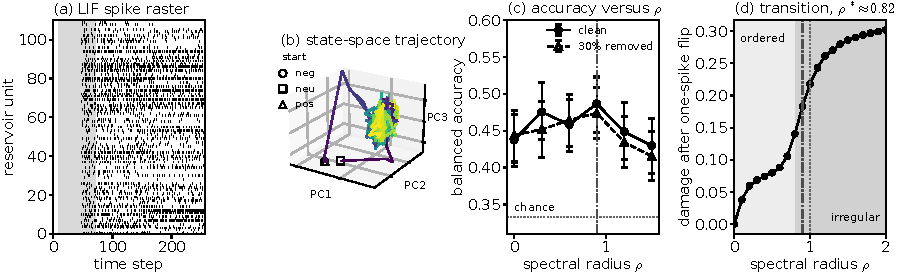
\includegraphics[width=\textwidth]{fig_reservoir_dyn.pdf}
\caption{The fixed LIF reservoir as a dynamical system, linked to accuracy. (a)~Spike raster (units $0$--$109$ of $256$) for one condition (shaded $=$ the $t\in[10,70)$ analysis window, about $-160$ to $+73$~ms around onset at step $51$). (b)~Population state-space trajectory (first three principal components of the $256$-unit membrane state), colored from epoch start (dark) to end (light), for the three affective conditions; the trajectories largely overlap, consistent with the modest clean separability. (c)~Subject-level BA ($95\%$ CI) versus spectral radius $\rho$, clean and with $30\%$ of electrodes removed; $\rho=0$ removes the recurrence, and the dash-dot line marks the pre-specified $\rho=0.9$. (d)~Damage-spreading order parameter versus $\rho$; shading separates the ordered and irregular regimes at the measured transition $\rho^\ast\approx0.82$; dash-dot $=$ $\rho=0.9$, dotted $=$ the echo-state heuristic $\rho=1$.}
\label{fig:resdyn}
\end{figure*}

\subsection{Baselines and Readout}
Two classical baselines are evaluated under the same subject-grouped protocol. The band-power baseline (A0) uses Welch band power in five bands ($1$--$4$, $4$--$8$, $8$--$13$, $13$--$30$, $30$--$45$~Hz) per channel ($5\times34=170$ dimensions). The ERP-window baseline (A0$_e$) uses mean amplitude in three fixed windows, about $-120$--$0$~ms (pre-stimulus baseline), $50$--$250$~ms (early components), and $250$--$600$~ms (P300 and late positive potential) relative to onset, per channel ($3 \times 34 = 102$ dimensions). The band-power, ERP-window, and reservoir representations use a balanced L2-regularized logistic readout to test separability without a high-capacity classifier.

As a trained deep baseline we evaluate EEGNet-8,2~\cite{lawhern2018eegnet} on the raw $34\times256$ ERP signal, trained per fold (Adam, $80$ epochs) with train-only per-channel standardization, with and without augmentation by random channel dropout and additive noise.

\subsection{Perturbation Diagnostics}
We separate two experiments. The feature-coordinate experiment (Sec.~\ref{sec:perturb}) suppresses a dropped channel's feature block after extraction and refills it by one of four rules; it isolates the fill convention and the coordinate origin, and applies to the fixed encoders. The signal-level experiment (Sec.~\ref{sec:rawsignal}) corrupts the test subjects' raw signal before any feature extraction, identically for every encoder including EEGNet with the same draws in each fold, while training uses the clean signal: removal of $10$, $30$, or $50\%$ of the electrodes, additive white noise at $5$~dB SNR per channel, and a uniform alignment shift of up to $\pm 50$~ms, with all features recomputed from the corrupted signal. In terms of Eq.~\eqref{eq:obs}, noise augments $\epsilon_t$, removal zeroes rows of $H$, and jitter shifts the sampling index of $x_t$. Performance is balanced accuracy (BA); Table~\ref{tab:clean} also reports macro-F1 and macro one-vs-rest ROC-AUC.

\subsection{Retention Scores and Two Confounds}
\label{sec:confound}
\emph{Raw retention}, the ratio of perturbed to clean BA, can overstate the stability of representations whose clean BA is close to chance ($c=1/3$ for three balanced classes), so we also report \emph{above-chance retention}, $(\mathrm{BA}_{\mathrm{pert}}-c)/(\mathrm{BA}_{\mathrm{clean}}-c)$.

Channel dropout also requires a fill rule for the dropped channel's features. We compare the common zero-fill convention with train-mean imputation, then add two in-distribution checks: train-fitted $k$-nearest-neighbor imputation ($k{=}10$) and a within-sample spatial fill using the mean of retained channels.

\emph{Non-invariance of zero-fill robustness.} Write the standardized readout input as $z=D_\sigma^{-1}(x-\mu)$ with $D_\sigma=\operatorname{diag}(\sigma)$, and let $S$ index the dropped coordinates. Zero-fill sets $x_S=0$, so the dropped block enters as $z_S=-D_{\sigma,S}^{-1}\mu_S$; train-mean fill sets $x_S=\mu_S$, so $z_S=0$. The two fills therefore differ by a fixed shift,
\begin{equation}\label{eq:noninv}
z_S^{\mathrm{zero}}-z_S^{\mathrm{mean}}=-D_{\sigma,S}^{-1}\mu_S .
\end{equation}

\noindent\textbf{Proposition 1.} \emph{Let the clean readout depend on $x$ only through $z$, so it is invariant to a constant offset $x\mapsto x-b$ (train-only standardization guarantees this). Then the clean prediction is unchanged by the re-centering, while the zero-fill dropout input shifts by $\Delta z_S=D_{\sigma,S}^{-1}b_S$. Hence the measured zero-fill dropout accuracy is not a function of the information in $x$ alone; it depends on the coordinate origin, and the zero- and mean-fill inputs coincide if and only if $\mu_S=0$.}

\noindent\emph{Proof.} Standardization subtracts the training mean, so $b$ cancels from the clean input. A zero-filled coordinate maps to $z_i=-(\mu_i-b_i)/\sigma_i$ instead of $-\mu_i/\sigma_i$, a shift of $b_i/\sigma_i\neq0$ for any $b_i\neq0$, and zero- and mean-fill coincide exactly when $\mu_S=0$.\hfill$\square$

For a linear readout with weights $w$, Eq.~\eqref{eq:noninv} changes the dropped-block contribution to the logit by $\sum_{i\in S} w_i\mu_i/\sigma_i$ between the two fills, at most $\lVert w_S\rVert\,\lVert D_{\sigma,S}^{-1}\mu_S\rVert$ in magnitude, so the fills can disagree only as far as the dropped features are non-centered, and only a centered code makes the choice immaterial. The reservoir's PCA code is near-centered: averaged over features and training folds, $|\mu_i|/\sigma_i$ is $0.06$ for the reservoir, against $0.75$ for ERP-window and $1.20$ for band-power, which is why it serves as a reference in Sec.~\ref{sec:perturb}.

\section{Experimental Protocol}
\subsection{Dataset and Task}
\label{sec:data}
The experiments use trial-averaged affective ERP data from the Stress, Health, and the Psychophysiology of Emotion (SHAPE) project~\cite{shape}, collected by the Laboratory for Clinical Affective Neuroscience at Stony Brook University, with 211 subjects after exclusion of one anomalous subject record. Each subject contributes three affective conditions (negative, neutral, pleasant), yielding 633 subject-condition observations. Each recorded epoch ($34$ scalp channels at $1024$~Hz, $1.2$~s, baseline-corrected over the $200$~ms pre-stimulus interval) is analyzed as every fourth of its first $1024$ samples: $256$ samples at $256$~Hz spanning $-200$ to $+800$~ms around stimulus onset (onset at sample $51$), z-scored per channel within each epoch; the grand averages show the expected late-positive-potential enhancement for emotional over neutral stimuli (Fig.~\ref{fig:erp}). Subject-level data are maintained in a restricted research environment; only aggregate, de-identified results are reported.

\begin{figure*}[t]
\centering
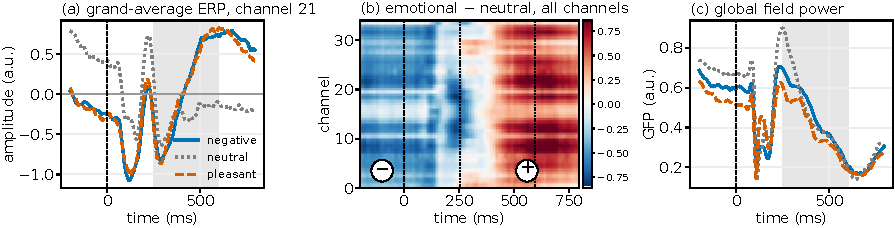
\includegraphics[width=0.92\textwidth]{fig_erp.pdf}
\caption{Trial-averaged affective ERP data (SHAPE cohort; grand averages over 211 subjects). (a)~Grand-average waveforms per condition at the most affect-discriminative channel; time $0$ $=$ stimulus onset (dashed), shaded $=$ the late ERP-window feature ($250$--$600$~ms). (b)~Spatiotemporal map of the emotional-minus-neutral difference across all $34$ channels (dotted $=$ the same window; $-$/$+$ mark the sign), showing the sustained LPP enhancement. (c)~Global field power per condition.}
\label{fig:erp}
\end{figure*}

\subsection{Validation}
All results share one fold structure, StratifiedGroupKFold (5 folds, seeds $42$--$46$) with subjects as groups, so observations from the same subject never span train and test; standardization is fitted on the training subjects, the fixed encoders use a balanced L2 logistic readout, and EEGNet is trained on the same folds. Uncertainty is estimated at the level of the subject, not the fold. For each representation we average the out-of-fold class probabilities of every observation across the five repeated partitions, then form $95\%$ confidence intervals (CIs) from $4000$ resamples of the $211$ subjects with replacement, keeping all three condition observations of a resampled subject together. Comparisons between encoders, fills, or conditions are paired differences under the same subject resampling. Because the five partitions are pooled into one prediction per observation before resampling, the dependence among the $25$ overlapping fold estimates, which reuse the same subjects, does not enter the intervals, and no test treats folds as independent samples. Chance is $1/3$, and a within-subject label-permutation null ($20$ permutations) gives mean BA $0.33$ to $0.34$ (SD at most $0.023$, maximum $0.39$) for every fixed encoder.

\section{Results}
\subsection{Clean Classification and Controls}
\label{sec:clean}
Table~\ref{tab:clean} reports clean three-class BA, macro-F1, and macro one-vs-rest ROC-AUC for the fixed encoders. ERP-window features are the strongest fixed encoder (BA $0.629$), above band-power ($0.494$) and the reservoir embedding ($0.487$), whose subject-level intervals overlap. EEGNet, trained on the raw signal under the same folds, is more accurate still (BA $0.731$, $[0.701,0.763]$; Table~\ref{tab:rawsignal}). The fixed encoders therefore carry genuine but modest condition information, and the reservoir is not the most accurate encoder.


\begin{table}[t]
\caption{Clean three-class balanced accuracy for the fixed encoders, with subject-level bootstrap $95\%$ CIs ($211$ subjects resampled with replacement, three conditions each), macro-F1, and macro one-vs-rest ROC-AUC from the pooled out-of-fold probabilities. Chance is $1/3$ (AUC $0.5$). EEGNet is in Table~\ref{tab:rawsignal}.}
\label{tab:clean}
\centering
\small
\setlength{\tabcolsep}{2.5pt}
\begin{tabular}{llccc}
\toprule
Cfg & Features & BA [95\% CI] & F1 & AUC \\
\midrule
A0$_e$ & ERP-window (102) & $0.629$ [$0.597$, $0.660$] & $0.629$ & $0.799$ \\
A0 & Band-power (170) & $0.494$ [$0.460$, $0.528$] & $0.492$ & $0.682$ \\
A1 & Reservoir \BSC{} (2176) & $0.487$ [$0.447$, $0.523$] & $0.485$ & $0.658$ \\
\bottomrule
\end{tabular}
\end{table}

\emph{Spectral radius and recurrent dynamics.} The recurrent dynamics contribute: relative to the pre-specified $\rho=0.9$, the feedforward layer ($\rho=0$) loses $0.049$ BA ($95\%$ CI $[-0.098,-0.002]$), and the strongly irregular $\rho=1.5$ loses $0.057$ ($[-0.106,-0.011]$; $-0.058$, $[-0.103,-0.016]$, with $30\%$ of electrodes removed; Fig.~\ref{fig:resdyn}c). Between $\rho=0.3$ and $1.2$ the differences from $\rho=0.9$ are within noise, as is the $\rho=0$ contrast with $30\%$ of electrodes removed ($-0.030$, $[-0.074,+0.016]$), so the optimum is broad rather than sharp. After an initial step at small $\rho$, the order parameter rises steadily, with its largest increment between $\rho=0.8$ and $0.9$ and saturation above $\rho\approx1.2$; its half-maximum crossing places the measured transition at $\rho^\ast\approx0.82$, below the echo-state heuristic $\rho=1$ (Fig.~\ref{fig:resdyn}d); the mean firing rate doubles across it ($0.06$ at $\rho=0.6$, $0.12$ at $\rho=0.9$). The pre-specified operating point thus lies just past the measured edge of the ordered regime, inside a broad accuracy optimum.

\emph{Temporal-binning ablation.} A single-bin total-count control (BSC$_1$) matches \BSC{}: the paired difference \BSC{} minus BSC$_1$ is $+0.001$ BA ($95\%$ CI $[-0.044,+0.047]$) on clean data and $-0.001$ ($[-0.046,+0.041]$) with $30\%$ of electrodes removed. The reservoir's accuracy comes from the fixed state-space expansion, not from six-bin temporal resolution, and we do not claim a temporal-coding benefit for \BSC{}.

\emph{Transduction and component controls.} Fitting the PCA basis on all subjects (transductive) instead of the training subjects gives BA $0.485$ $[0.447,0.521]$, against $0.487$, and $16$, $32$, $64$, or $128$ components per electrode give $0.477$ to $0.507$, all inside the $64$-component interval $[0.447,0.523]$. Neither the basis nor the component count accounts for the results.

\subsection{Feature-Coordinate Experiment: Two Scoring Confounds}
\label{sec:perturb}
Channel dropout is where the reported conclusion depends on the scoring convention (Table~\ref{tab:dropconf}, Fig.~\ref{fig:impute}).

\emph{Accuracy-floor effect.} Raw retention makes the reservoir look the most robust encoder: at $30\%$ dropout its BA does not move (retention $1.00$, against $0.85$ for ERP-window under zero-fill). This reflects the ratio, not stability: the reservoir sits close to the $1/3$ chance floor and has little above-chance accuracy to lose. Above-chance retention corrects the floor, but its denominator is only about $0.15$ for the reservoir, so it is unstable near chance and can exceed one. We therefore treat absolute BA and paired subject-level differences as primary, with retention ratios as secondary diagnostics.

\emph{Zero-imputation effect.} By Proposition~1 the two constant fills can disagree only through the non-centeredness of the dropped features, and the subject-level gaps are ordered as that non-centeredness is (Fig.~\ref{fig:impute}a). At $30\%$ dropout, mean-fill exceeds zero-fill by $+0.055$ BA ($95\%$ CI $[+0.024,+0.087]$) for band-power and by $+0.042$ ($[+0.011,+0.074]$) for ERP-window, but by $-0.000$ ($[-0.022,+0.022]$) for the near-centered reservoir. Across rates from $10$ to $50\%$ the reservoir's two constant-fill scores agree within $0.016$ BA and no CI excludes zero, whereas the gap of the non-centered encoders varies with the rate and is significant for band-power at $20$ and $30\%$ and for ERP-window at $30\%$. $k$NN fill differs in kind (Fig.~\ref{fig:impute}b): it replaces the dropped block by an average over ten training neighbors, which adds content rather than moving the origin, and at $40$ and $50\%$ it significantly raises every encoder, ERP-window most ($+0.13$ BA at $50\%$, $[+0.09,+0.16]$).

\emph{Encoder comparison.} ERP-window features lead the reservoir under every fill, but the fill sets the size of the lead (Table~\ref{tab:dropconf}). At $30\%$ dropout the paired difference ERP-window minus reservoir is $+0.049$ BA under zero-fill ($95\%$ CI $[+0.003,+0.095]$) and $+0.092$ to $+0.107$ under the three in-distribution fills, whose CIs all lie above $+0.04$. Zero-fill thus halves the measured advantage of the strongest fixed encoder, because only the non-centered encoder's score moves with the constant.

\begin{table}[t]
\caption{Channel dropout at $30\%$ (feature-coordinate experiment): subject-level balanced accuracy for the fixed encoders under four fill rules, and the paired difference ERP-window minus reservoir under the same subject resampling. A positive difference whose $95\%$ CI excludes zero means ERP-window is significantly ahead. Per-encoder $95\%$ CIs are $\pm0.03$ to $\pm0.04$.}
\label{tab:dropconf}
\centering
\small
\setlength{\tabcolsep}{2.5pt}
\begin{tabular}{lcccc}
\toprule
Fill & Band-pow. & ERP-win. & Reserv. & ERP$-$Res [95\% CI] \\
\midrule
Zero & $0.417$ & $0.536$ & $0.487$ & $+0.049$ [$+0.003,+0.095$] \\
Mean & $0.472$ & $0.578$ & $0.487$ & $+0.092$ [$+0.049,+0.134$] \\
$k$NN & $0.483$ & $0.610$ & $0.507$ & $+0.103$ [$+0.062,+0.147$] \\
Spatial & $0.488$ & $0.589$ & $0.482$ & $+0.107$ [$+0.063,+0.150$] \\
\bottomrule
\end{tabular}
\end{table}

\begin{figure}[t]
\centering
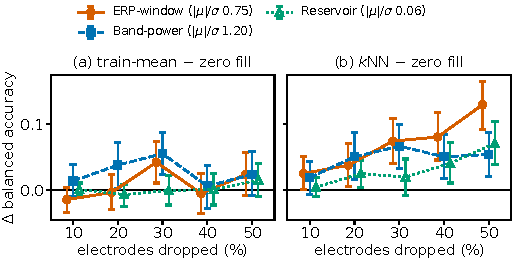
\includegraphics[width=\columnwidth]{fig_impute_subj.pdf}
\caption{How much the fill rule alone moves channel-dropout accuracy (feature-coordinate experiment): paired subject-level change in BA relative to zero-fill, with $95\%$ CIs, versus the share of electrodes dropped. (a)~Train-mean fill, which differs from zero-fill only by the shift of Eq.~\eqref{eq:noninv}; the legend gives the mean $|\mu|/\sigma$ of each encoder's features. (b)~$k$NN fill, which replaces the dropped block by an average of ten training neighbors and so changes its content.}
\label{fig:impute}
\end{figure}

\subsection{Signal-Level Perturbations}
\label{sec:rawsignal}
The signal-level experiment asks what happens when the recorded signal itself is corrupted (Table~\ref{tab:rawsignal}). A removed electrode contributes zero band-power and zero ERP amplitude, so for these two encoders removal is exactly zero-fill, and their removal rows equal the zero-fill scores of Sec.~\ref{sec:perturb}. For the reservoir, a silent electrode yields a zero spike-count block, which projects to the negative of the projected training mean rather than to the PCA origin, so the shift of Eq.~\eqref{eq:noninv} reappears before the projection.

Three results stand out. First, ERP-window features remain the most accurate fixed encoder under every condition; their paired lead over the reservoir ranges from $+0.06$ to $+0.14$ BA, and every CI excludes zero. Second, the reservoir holds its accuracy through $30\%$ removal (loss $0.013$, $95\%$ CI $[-0.014,+0.041]$) but falls to $0.393$ at $50\%$, close to chance (loss $0.093$, $[+0.055,+0.131]$), so its fill invariance is a property of its feature space, not robustness to missing electrodes. Third, $5$~dB noise costs band-power $0.059$ BA ($[+0.019,+0.098]$) while ERP-window and the reservoir stay within noise of their clean scores, and $\pm50$~ms jitter moves no fixed encoder, consistent with the wide ERP windows and with the single-bin control of Sec.~\ref{sec:clean}.

\emph{Training effect.} EEGNet ingests the same corrupted signal and is the most accurate encoder in every condition (clean BA $0.731$, $95\%$ CI $[0.701,0.763]$; paired lead over ERP-window $+0.08$ to $+0.20$, every CI excluding zero). Unaugmented, it loses $0.071$ BA at $30\%$ removal and $0.144$ at $50\%$, close to the ERP-window losses ($0.093$ and $0.155$). Training with channel-dropout and noise augmentation leaves clean accuracy unchanged (paired difference $-0.000$, $[-0.025,+0.022]$) and cuts these losses by more than half, to $0.028$ and $0.062$: the augmented network is ahead by $+0.043$ ($[+0.009,+0.077]$) at $30\%$ and $+0.082$ ($[+0.049,+0.115]$) at $50\%$, while neither variant loses more than $0.024$ BA to noise or jitter. For this architecture, accuracy under electrode loss is thus set mainly by the training procedure (Fig.~\ref{fig:deapaug}b).

\begin{table}[t]
\caption{Signal-level perturbations: subject-level balanced accuracy with every representation recomputed from the corrupted test signal (same draws for all encoders; training on clean data, EEGNet also with augmentation). Per-cell $95\%$ CIs are $\pm0.03$ to $\pm0.04$. Chance is $1/3$.}
\label{tab:rawsignal}
\centering
\small
\setlength{\tabcolsep}{3pt}
\begin{tabular}{lccccc}
\toprule
Condition & Band-pow. & ERP-win. & Reserv. & EEGNet & +aug. \\
\midrule
Clean & $0.494$ & $0.629$ & $0.487$ & $0.731$ & $0.731$ \\
$10\%$ removed & $0.476$ & $0.602$ & $0.469$ & $0.719$ & $0.722$ \\
$30\%$ removed & $0.417$ & $0.536$ & $0.474$ & $0.660$ & $0.703$ \\
$50\%$ removed & $0.450$ & $0.474$ & $0.393$ & $0.588$ & $0.670$ \\
Noise $5$~dB & $0.436$ & $0.619$ & $0.479$ & $0.738$ & $0.727$ \\
Jitter $\pm50$~ms & $0.496$ & $0.626$ & $0.493$ & $0.719$ & $0.708$ \\
\bottomrule
\end{tabular}
\end{table}

\subsection{External Replication on an Independent Affective Dataset}
\label{sec:deap}
On DEAP~\cite{koelstra2012deap} (32 subjects, band-power features, binary valence, within-subject $5$-fold), the same pattern appears and is larger (Fig.~\ref{fig:deapaug}a): at $30\%$ dropout the same features score BA $0.540$ under zero-fill ($95\%$ CI $[0.528, 0.552]$) but $0.621$ $[0.591, 0.648]$ under mean and $0.638$ $[0.607, 0.668]$ under $k$NN fill, with CIs from resampling the $32$ subjects' mean BA. With clean BA $0.639$, the fill rule alone moves measured accuracy under dropout by up to $0.11$ BA, on a second dataset, task, and montage. This is an external check of the fill-rule effect, not a replication of the full comparison.

\begin{figure}[t]
\centering
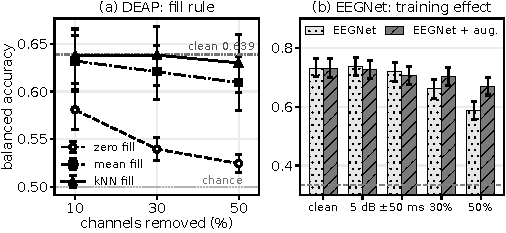
\includegraphics[width=\columnwidth]{fig_deap_aug.pdf}
\caption{(a)~External check on DEAP~\cite{koelstra2012deap} (32 subjects, within-subject binary valence, band-power; clean BA $0.639$; CIs from resampling subjects). Under channel removal, BA depends strongly on the fill rule. (b)~EEGNet without and with channel-dropout and noise augmentation under the signal-level conditions of Table~\ref{tab:rawsignal} (clean, $5$~dB noise, $\pm50$~ms jitter, $30\%$ and $50\%$ of electrodes removed; subject-level $95\%$ CIs). Augmentation leaves clean accuracy unchanged, moves noise and jitter accuracy by at most $0.011$, and cuts the loss to electrode removal by more than half.}
\label{fig:deapaug}
\end{figure}

\section{Discussion}
The main result is methodological: raw retention favors encoders near the chance floor, zero-imputation penalizes non-centered features after standardization, and for trained models augmentation is a third factor. The zero-fill effect agrees with the benchmark finding that channel-dropout fragility depends on whether dropped channels are removed or zero-padded~\cite{sirca2026beyond}, and Proposition~1 gives its mechanism for standardized features. After accounting for these choices, the fixed reservoir should not be described as the most channel-robust encoder: ERP-window features lead it under every fill at $30\%$ dropout and under every signal-level condition, and zero-fill halves that lead. The reservoir remains useful as a near-centered reference that makes the effect in the other encoders visible, but its invariance belongs to its feature space and does not survive signal-level removal of half the electrodes. Its dynamics still matter: removing the recurrence or driving the reservoir into the irregular regime lowers accuracy, and the pre-specified operating point lies near the measured edge of the ordered regime, in line with edge-of-chaos results for other reservoirs~\cite{bertschinger2004realtime,legenstein2007edge}.

Learned and generative imputation sit further along the same spectrum (Sec.~\ref{sec:related}). If non-learned fills, constant or $k$NN, already move measured accuracy by up to $0.13$ BA and halve an encoder difference, the fill model of a learned imputer is part of the measured result and should be reported with it. These results suggest a minimal reporting standard: report absolute accuracy with subject-level uncertainty, state and vary the channel-fill rule, and report trained-model results with and without augmentation~\cite{rommel2022augment}.

\textbf{Limitations.} The primary cohort is a single trial-averaged affective-ERP dataset. The imputation effect nevertheless follows from the standardization algebra of Eq.~\eqref{eq:noninv} and is observed across fill rules, dropout rates, and the independent DEAP check, but paradigm-matched multi-cohort ERP validation would strengthen it. EEGNet is trained with one fixed recipe, without a hyperparameter search, and the spectral-radius sweep uses a single draw of the reservoir weights. Adversarial attacks and montage shifts are not evaluated, and graph topology and structure--function coupling are outside the scope of this paper.

\section{Conclusion}
Channel-dropout robustness rankings for affective-ERP representations depend on the scoring protocol. Raw retention can overstate robustness near the chance floor, zero-imputation shifts non-centered features after standardization and here halves the measured lead of the strongest fixed encoder, and trained models need their augmentation state made explicit. The fixed spiking reservoir, operated near its measured edge of stability, is not the most accurate encoder, but its near-centered code makes these protocol effects visible, and the fill-rule effect replicates on DEAP.

\textbf{Ethics.} The SHAPE study was collected by the Stony Brook University Laboratory for Clinical Affective Neuroscience under that laboratory's Institutional Review Board oversight. DEAP is a publicly released dataset governed by its original collection protocol~\cite{koelstra2012deap}.

\textbf{Data Availability.} For information on the SHAPE study dataset, contact the Laboratory for Clinical Affective Neuroscience at Stony Brook University~\cite{shape}. DEAP is public~\cite{koelstra2012deap}.

\IEEEtriggeratref{16}
\begin{thebibliography}{99}

\bibitem{maass2002real}
W. Maass, T. Natschl\"ager, and H. Markram, ``Real-time computing without stable states: A new framework for neural computation based on perturbations,'' \emph{Neural Computation}, vol. 14, no. 11, pp. 2531--2560, 2002.

\bibitem{jaeger2001echo}
H. Jaeger, ``The echo state approach to analysing and training recurrent neural networks,'' German National Research Center for Information Technology, GMD Report 148, 2001.

\bibitem{jaeger2004harnessing}
H. Jaeger and H. Haas, ``Harnessing nonlinearity: Predicting chaotic systems and saving energy in wireless communication,'' \emph{Science}, vol. 304, no. 5667, pp. 78--80, 2004.

\bibitem{lukosevicius2009reservoir}
M. Luko\v{s}evi\v{c}ius and H. Jaeger, ``Reservoir computing approaches to recurrent neural network training,'' \emph{Computer Science Review}, vol. 3, no. 3, pp. 127--149, 2009.

\bibitem{bertschinger2004realtime}
N. Bertschinger and T. Natschl\"ager, ``Real-time computation at the edge of chaos in recurrent neural networks,'' \emph{Neural Computation}, vol. 16, no. 7, pp. 1413--1436, 2004.

\bibitem{legenstein2007edge}
R. Legenstein and W. Maass, ``Edge of chaos and prediction of computational performance for neural circuit models,'' \emph{Neural Networks}, vol. 20, no. 3, pp. 323--334, 2007.

\bibitem{diehl2015unsupervised}
P. U. Diehl and M. Cook, ``Unsupervised learning of digit recognition using spike-timing-dependent plasticity,'' \emph{Frontiers in Computational Neuroscience}, vol. 9, Art. no. 99, 2015.

\bibitem{roy2019towards}
K. Roy, A. Jaiswal, and P. Panda, ``Towards spike-based machine intelligence with neuromorphic computing,'' \emph{Nature}, vol. 575, no. 7784, pp. 607--617, 2019.

\bibitem{lane2023arspi}
A. Lane, W. Tang, and B. Nelson, ``Towards ARSPI-Net: Development of an efficient hybrid deep learning framework,'' in \emph{Proc. IEEE Long Island Systems, Applications and Technology Conf. (LISAT)}, Old Westbury, NY, USA, 2023, pp. 1--8.

\bibitem{lane2024arspi}
A. Lane, W. Tang, and B. Nelson, ``Towards ARSPI-Net: Advancing EEG feature extraction with neuromorphic algorithms,'' in \emph{Proc. IEEE Long Island Systems, Applications and Technology Conf. (LISAT)}, Holtsville, NY, USA, 2024, pp. 1--8.

\bibitem{gong2023sglnet}
P. Gong, P. Wang, Y. Zhou, and D. Zhang, ``A spiking neural network with adaptive graph convolution and LSTM for EEG-based brain-computer interfaces,'' \emph{IEEE Trans. Neural Syst. Rehabil. Eng.}, vol. 31, pp. 1440--1450, 2023.

\bibitem{hjorth1970eeg}
B. Hjorth, ``EEG analysis based on time domain properties,'' \emph{Electroencephalography and Clinical Neurophysiology}, vol. 29, no. 3, pp. 306--310, 1970.

\bibitem{subasi2007eeg}
A. Subasi, ``EEG signal classification using wavelet feature extraction and a mixture of expert model,'' \emph{Expert Systems with Applications}, vol. 32, no. 4, pp. 1084--1093, 2007.

\bibitem{makeig2002dynamic}
S. Makeig, M. Westerfield, T.-P. Jung, S. Enghoff, J. Townsend, E. Courchesne, and T. J. Sejnowski, ``Dynamic brain sources of visual evoked responses,'' \emph{Science}, vol. 295, no. 5555, pp. 690--694, 2002.

\bibitem{blankertz2011singletrial}
B. Blankertz, S. Lemm, M. Treder, S. Haufe, and K.-R. M\"uller, ``Single-trial analysis and classification of ERP components: a tutorial,'' \emph{NeuroImage}, vol. 56, no. 2, pp. 814--825, 2011.

\bibitem{lawhern2018eegnet}
V. J. Lawhern, A. J. Solon, N. R. Waytowich, S. M. Gordon, C. P. Hung, and B. J. Lance, ``EEGNet: A compact convolutional neural network for EEG-based brain-computer interfaces,'' \emph{Journal of Neural Engineering}, vol. 15, no. 5, 056013, 2018.

\bibitem{craik2019deep}
A. Craik, Y. He, and J. L. Contreras-Vidal, ``Deep learning for electroencephalogram (EEG) classification tasks: A review,'' \emph{Journal of Neural Engineering}, vol. 16, no. 3, 031001, 2019.

\bibitem{chiang2023depression}
H.-S. Chiang, M.-Y. Chen, and L.-S. Liao, ``Cognitive depression detection cyber-medical system based on EEG analysis and deep learning approaches,'' \emph{IEEE J. Biomed. Health Inform.}, vol. 27, no. 2, pp. 608--616, 2023.

\bibitem{guo2025mma}
Y. Guo, K. Yang, and Y. Wu, ``A multi-modality attention network for driver fatigue detection based on frontal EEG, EDA and PPG signals,'' \emph{IEEE J. Biomed. Health Inform.}, vol. 29, no. 6, pp. 4009--4022, 2025.

\bibitem{delpup2025preprocessing}
F. Del Pup, A. Zanola, L. F. Tshimanga, A. Bertoldo, and M. Atzori, ``The more, the better? Evaluating the role of EEG preprocessing for deep learning applications,'' \emph{IEEE Trans. Neural Syst. Rehabil. Eng.}, vol. 33, pp. 1061--1070, 2025.

\bibitem{kornblith2019similarity}
S. Kornblith, M. Norouzi, H. Lee, and G. Hinton, ``Similarity of neural network representations revisited,'' in \emph{Proc. Int. Conf. Machine Learning}, 2019, pp. 3519--3529.

\bibitem{sirca2026beyond}
U. \v{S}irca, M. Alimardani, S. Zafeiriou, and K. Barmpas, ``Beyond accuracy: Robustness, interpretability and expressiveness of EEG foundation models,'' \emph{arXiv:2605.17562}, 2026.

\bibitem{banville2022dsf}
H. Banville, S. U. N. Wood, C. Aimone, D.-A. Engemann, and A. Gramfort, ``Robust learning from corrupted EEG with dynamic spatial filtering,'' \emph{NeuroImage}, vol. 251, 118994, 2022.

\bibitem{rommel2022augment}
C. Rommel, J. Paillard, T. Moreau, and A. Gramfort, ``Data augmentation for learning predictive models on EEG: A systematic comparison,'' \emph{Journal of Neural Engineering}, vol. 19, no. 6, 066020, 2022.

\bibitem{perrin1989spherical}
F. Perrin, J. Pernier, O. Bertrand, and J. F. Echallier, ``Spherical splines for scalp potential and current density mapping,'' \emph{Electroencephalography and Clinical Neurophysiology}, vol. 72, no. 2, pp. 184--187, 1989.

\bibitem{bi2024graymatters}
Y. Bi, A. Abrol, S. Jia, J. Sui, and V. D. Calhoun, ``Gray matters: ViT-GAN framework for identifying schizophrenia biomarkers linking structural MRI and functional network connectivity,'' \emph{NeuroImage}, vol. 297, 120674, 2024.

\bibitem{hu2025gmldm}
X. Hu, J. Yang, S. Jia, Y. Bi, and V. D. Calhoun, ``GM-LDM: Latent diffusion model for brain biomarker identification through functional data-driven gray matter synthesis,'' arXiv:2506.12719, 2025.

\bibitem{koelstra2012deap}
S. Koelstra \emph{et al.}, ``DEAP: A database for emotion analysis using physiological signals,'' \emph{IEEE Trans. Affective Computing}, vol. 3, no. 1, pp. 18--31, 2012.

\bibitem{shape}
Laboratory for Clinical Affective Neuroscience, ``The Stress, Health, and the Psychophysiology of Emotion (SHAPE) project,'' Stony Brook University, Stony Brook, NY, USA. [Online]. Available: \url{https://lab-can.com}

\end{thebibliography}

\end{document}